\documentclass[preprint, 3p,
authoryear]{elsarticle} %review=doublespace preprint=single 5p=2 column
%%% Begin My package additions %%%%%%%%%%%%%%%%%%%

\usepackage[hyphens]{url}

  \journal{MU journals} % Sets Journal name

\usepackage{graphicx}
%%%%%%%%%%%%%%%% end my additions to header

\usepackage[T1]{fontenc}
\usepackage{lmodern}
\usepackage{amssymb,amsmath}
% TODO: Currently lineno needs to be loaded after amsmath because of conflict
% https://github.com/latex-lineno/lineno/issues/5
\usepackage{lineno} % add
\usepackage{ifxetex,ifluatex}
\usepackage{fixltx2e} % provides \textsubscript
% use upquote if available, for straight quotes in verbatim environments
\IfFileExists{upquote.sty}{\usepackage{upquote}}{}
\ifnum 0\ifxetex 1\fi\ifluatex 1\fi=0 % if pdftex
  \usepackage[utf8]{inputenc}
\else % if luatex or xelatex
  \usepackage{fontspec}
  \ifxetex
    \usepackage{xltxtra,xunicode}
  \fi
  \defaultfontfeatures{Mapping=tex-text,Scale=MatchLowercase}
  \newcommand{\euro}{€}
\fi
% use microtype if available
\IfFileExists{microtype.sty}{\usepackage{microtype}}{}
\usepackage[]{natbib}
\bibliographystyle{elsarticle-harv}

\usepackage{graphicx}
\ifxetex
  \usepackage[setpagesize=false, % page size defined by xetex
              unicode=false, % unicode breaks when used with xetex
              xetex]{hyperref}
\else
  \usepackage[unicode=true]{hyperref}
\fi
\hypersetup{breaklinks=true,
            bookmarks=true,
            pdfauthor={},
            pdftitle={The Impact of Fintech Develoment on the Financial Inclusion Gender Gap (FIGG) in Sub-Saharan African (SSA) countries.},
            colorlinks=false,
            urlcolor=blue,
            linkcolor=magenta,
            pdfborder={0 0 0}}

\setcounter{secnumdepth}{5}
% Pandoc toggle for numbering sections (defaults to be off)


% tightlist command for lists without linebreak
\providecommand{\tightlist}{%
  \setlength{\itemsep}{0pt}\setlength{\parskip}{0pt}}




\usepackage{float}
\usepackage{graphicx}
\usepackage{subcaption}



\begin{document}


\begin{frontmatter}

  \title{The Impact of Fintech Develoment on the Financial Inclusion
Gender Gap (FIGG) in Sub-Saharan African (SSA) countries.}
    \author[Department of Statistics, Miami University]{Simon Atoyire%
  %
  }
   \ead{atoyirs@miamioh.edu} 
      \affiliation[]{
    organization={Department of Statistics, Miami
University},addressline={501 E High
Street},city={Oxford},postcode={45056},state={Ohio},country={United
States},}
    \cortext[cor1]{Corresponding author}
    \fntext[]{Department of Statistics, Miami University.}
  
  \begin{abstract}
  Development of financial inclusion and gender diversity has gained
  attention all over the world and this has resulted in international
  bodies such as the United Nations initiate 17 sustainable development
  goals with Goals 1 and 5 focused on eradicating poverty and promoting
  gender equality respectively. These issues still remain persistent in
  developing countries, especially eradicating the gender gap in
  financial inclusion. This paper therefore investigates how Fintech
  could influence the financial inclusion gender gap in Sub-saharan
  Africa through data visualization. Data on Fintch development and
  Financial Inclusion gender gap (FIGG) was obtained from the the Global
  Findex database and the World bank world development indicators
  database for 2011, 2014, 2017, and 2021. The study used time series
  plots, chloropleths, bar plots and scatter plots for the analysis.

  The result from the time series plot supports the growing trend of
  FIGG in the SSA region suggested by the World Bank. Th finding also
  showed that Fintech development in SSA has a positive linear
  relationship with gender gap associatd with loan accessibility, a
  negative linear relationship with gender gap associated with account
  ownership and an almost neutral relationship with the gender gap
  associated with savings. The study also found that most of the SSA
  countries studied are similar in terms of the magnitude of financial
  inclusion gender gap. three dependent (Fintech) variables - access to
  internet, access to electricity, and mobile telephony ar highly
  correlated. Thus, further empirical investigation such as regression
  analysis is recommended to provide in-depth understanding of the
  association.
  \end{abstract}
    \begin{keyword}
    Financial Inclusion \sep Gender Gap \sep Financial inclusion gender
gap \sep Fintech \sep Development \sep 
    Sub-Saharan Africa
  \end{keyword}
  
 \end{frontmatter}

\hypertarget{introduction}{%
\section{INTRODUCTION}\label{introduction}}

\citet{banna2022fintech} argue that Financial Technology (Fintech) is
one of the most promising technologies because it has the potential to
address issues of inequality, poverty, and the lack of access to
financial services in Africa. According to \citet{board2020financial},
the Financial Stability Board (FSB) defines Fintech as a set of
technology that facilitates new and improved financial services
(including new apps, products, business models, and procedures) for
everyone from corporations to individual consumers. With the emergence
and adoption of Fintech in Africa, financial market participants both
men and women now have more potential to access and use quality
financial services which is also as a result of the increasing
participation of financial institutions in Fintech solutions. Fintech is
more widely used in the West and East Asia, but in Sub-Saharan Africa it
has just recently begun to gain traction as a means to expand access to
financial services and help the region's impoverished. More than a
decade-long investment in ICT in SSA countries has paved the way for
Fintech-based financial inclusion, and the quick penetration and
acceptance of the technology among financial market stakeholders have
made it a reality according to \citet{tchamyou2019role}.

\bigskip

Development of financial inclusion and gender diversity has gained
attention all over the world and this has resulted in international
bodies such as the United Nations initiate Sustainable Development Goals
1 and 5 focused on eradicating poverty and promoting gender equality
respectively. This issue remains in developing countries, particularly
in sub-Saharan Africa (SSA), hinted by \citet{demirguc2018global},
despite the acknowledgement of the importance of female financial
inclusion for both economic and sustainable development.
\citet{adegbite2020bridging} still identify eradicating the gender gap
in financial inclusion as a top priority for the 21st century, which is
especially true for SSA, where the financial inclusion gender gap
appears to be high. In contrast to the dramatic reductions in gender
gaps in access to financial services seen in countries with high and
middle incomes, \citet{Ferrer2023Sub-Saharan} argues that the case in
SSA is found to widen from its previous 7\% in 2011 to 12\% in 2021.
With the global financial inclusion gender gap standing at 4\% according
to the 2021 Global Findex Database, that of SSA stands at 12\%. This
highlights how much work and how urgent it is for the region to reduce
this gap. This paper therefore investigates how Fintech could influence
the financial inclusion gender gap in Sub-saharan Africa through data
visualization.

\hypertarget{data-and-method}{%
\section{DATA AND METHOD}\label{data-and-method}}

To examine the relationship between FIGG and FinTech, quantitative data
was obtained for a sample of 30 Sub-Saharan African Countries for the
periods 2011, 2014, 2017 and 2021. These time points were selected
strategically as these are the periods in which Financial Inclusion Data
were collected by the World bank. The data was analysed using data
visualization. The data included the level of financial inclusion and
FinTech use in each of the 30 countries.

\bigskip

\hypertarget{independent-variable}{%
\subsection{Independent Variable}\label{independent-variable}}

Since the use of Fintech is impossible without access to electricity,
this paper just like \citet{chen2023fintech} and
\citet{demir2022fintech} used mobile telephony and internet access
together with access to electricity as used by
\citet{yeyouomo2023fintechs} to measure of Fintech develoment. However,
access to electricity influences access to internet and the use of
mobile phones, hence there is correlation between these three variables
and thus using them together in the same model as done by Yeyouomo et
al.~(2023) would result in multicollinearity and makes the model
inappropriate. This could lead to unstable estimates, reduced precision,
and difficulty in interpreting results, thus providing unclear
information about the effect of Fintech on the various FIGG variables.
To deal with this issue, Fintech development is approximated by a single
variable obtained by weighing the effect of each of the Fintech
variables on FIGG and computing the weighted average. This single
Fintech variable considers the effects of all the three variables.

\hypertarget{dependent-variable}{%
\subsection{Dependent Variable}\label{dependent-variable}}

To measure FIGG, data on the proportion of men and women who have access
to and use financial services was collected from the World Bank Global
Findex Database. FIGG is often quantified by examining the disparity
between men and women in their use of and access to financial services,
which is in accordance with \citet{adegbite2020bridging} and
\citet{tok2022fintech}. In this vein, Yeyouomo et al.~(2023) computed
FIGG as the difference between males and females with access to
financial services. Although this is a good measure, the absolute
difference fails to provide an accurate comparison between countries.
Countries with wide absolute difference may appear to have higher gender
gaps which may not be the case due to the difference in population of
males and females. To deal with this issue, the current study computes
gender gap as the ratio of the difference to the total proportion of
males and females with access to financial services. This standardizes
the gender gap to promote comparison. With these modifications, the
current study examines the impact of Fintech on financial inclusion
gender gap in SSA to provide a more nuanced set of results than has been
achieved in previous studies. A negative value indicates more women than
men and a positive value indicates otherwise. The variables description
table below provides information on how the variables were measured and
their sources.

\begin{figure}[ht]
  \centering
  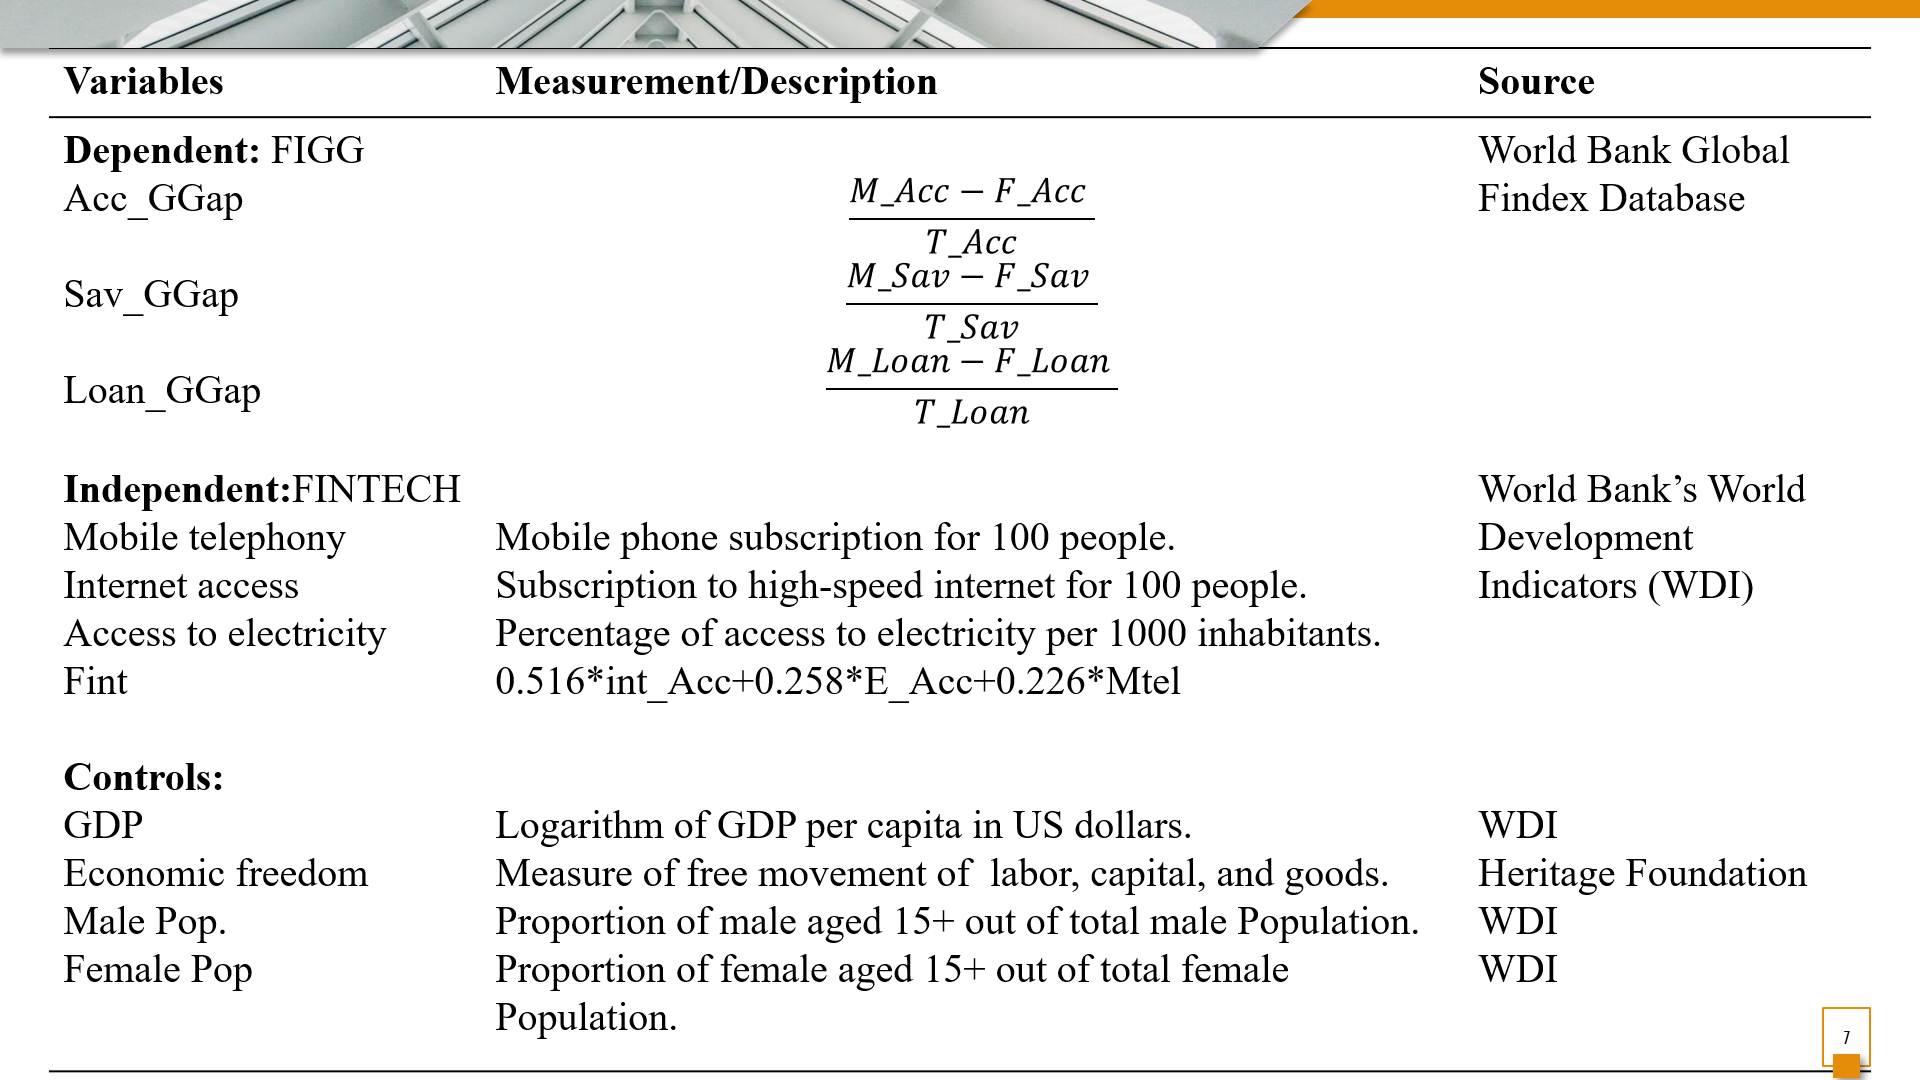
\includegraphics[width=0.8\textwidth]{Var.Desc.Table.png}
  \caption{Variable Description Table}
  \label{fig:fig1}
  \textbf{Source:} Created by Author.
\end{figure}

\bigskip

where:

\vspace{1pt}

M\_Acc = proportion of males aged 15+ who have an account with formal
financial Inst or mobile money;

\vspace{1pt}

F\_Acc = proportion of females aged 15+ who have an account with formal
financial Inst or mobile money;

\vspace{1pt}

T\_Acc = Total proportion of males and females aged 15+ who have an
account with formal financial Institution or mobile money;

\vspace{1pt}

M\_Sav = proportion of males aged 15+ who saved some money with a
financial institution in the past year; \vspace{1pt}

F\_Sav = proportion of females aged 15+ who saved some money with
financial institutions in the past year;

\vspace{1pt}

T\_Sav = Total proportion of males and females aged 15+ who saved some
money with financial institutions in the past year;

\vspace{1pt}

M\_Loan = proportion of males aged 15+ who obtained loans from financial
institutions in the past year;

\vspace{1pt}

F\_Loan = proportion of females aged 15+ who obtained loans from
financial institutions in the past year; \vspace{1pt}

T\_Loan = Total proportion of males and females aged 15+ who obtained
loans from financial institutions in the past year;

\vspace{1pt}

Fint = composite Fintech Development.

\hypertarget{analysis}{%
\section{ANALYSIS}\label{analysis}}

\hypertarget{yearly-financial-inclusion-gender-gap}{%
\subsection{Yearly Financial Inclusion Gender
Gap}\label{yearly-financial-inclusion-gender-gap}}

In studying financial inclusion in the Sub-Saharan region, the trend of
financial inclusion for males and females in the region was observed.
Financial inclusion in the area was found to be improving steadily in
the region as all the three variables showed appreciation over the years
for both males and females. Savings, however, recorded a decline for
both genders between 2014 and 2017 as shown in fig.2. This decline
appeared to be consistent with the decline in average GDP in the area
and the slight decline in employment rate figures 5 and 4 respectively.
This is not surprising as the African continent during the same period
experienced some economic difficulties caused by but not limited to the
outbreak of Ebola in West Africa, political instability and conflict in
countries such as Nigeria, Somalia, Democratic Republic of the Congo
(DRC), Central African Republic (CAR), South Sudan, Mali, and Burundi,
just to mention a few, significant currency depreciation in many
countries (including Ghana, Nigeria, South Africa, Zimbabwe, Zambia, and
Angola). These economic issues led to low GDP which could explain the
reason for the decline in savings as there was not much for citizens to
save considering the hike in commodity prices with fairly no increase in
salaries as well as low income. In addition, although financial
inclusion seem to be improving in the SSA, it is still low considering
that it is still lower than 50\% for both males and females. The worst
of the three is financial inclusion in terms of loan accessibility. As
at 2021, the proportion of males and females that have access to credit
from formal financial institutions was below 15\%. The study also found
that the gap between male and female for account ownership, savings, and
loan accessibility continually widened over the year with the gap
standing at above 5\% in 2021 for each of the financial inclusion
indexes.

\bigskip

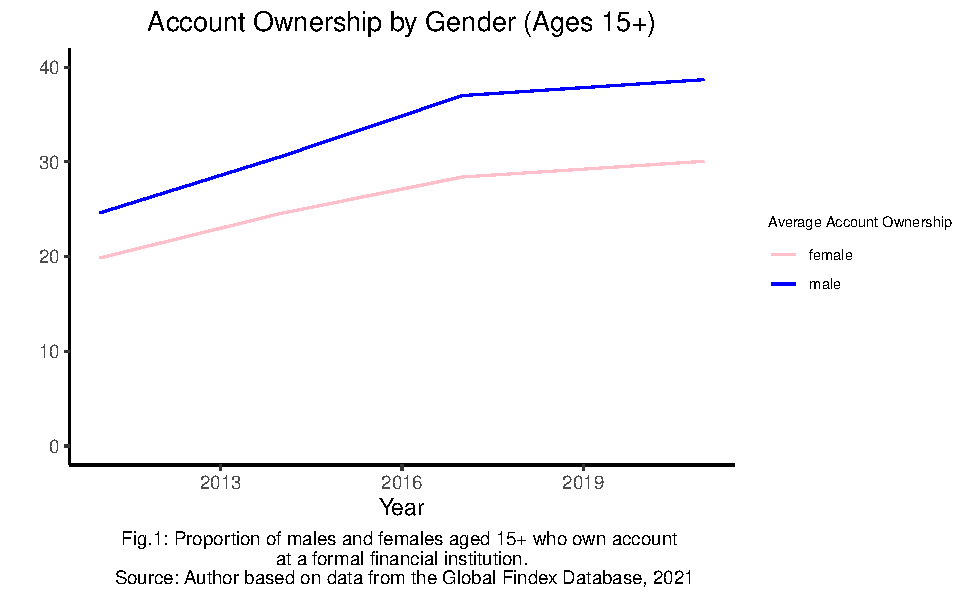
\includegraphics{504.Project1_files/figure-latex/unnamed-chunk-3-1.pdf}
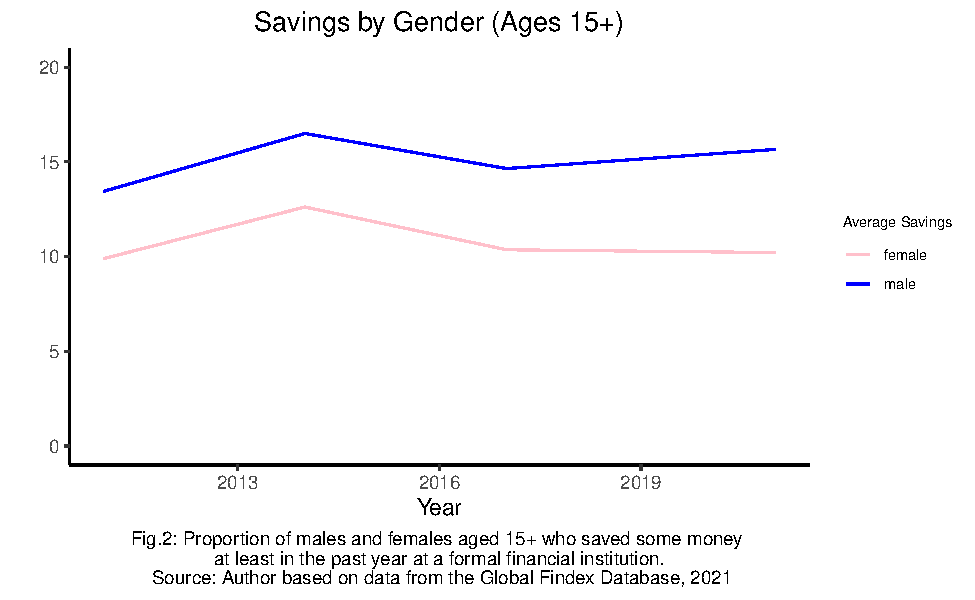
\includegraphics{504.Project1_files/figure-latex/unnamed-chunk-3-2.pdf}
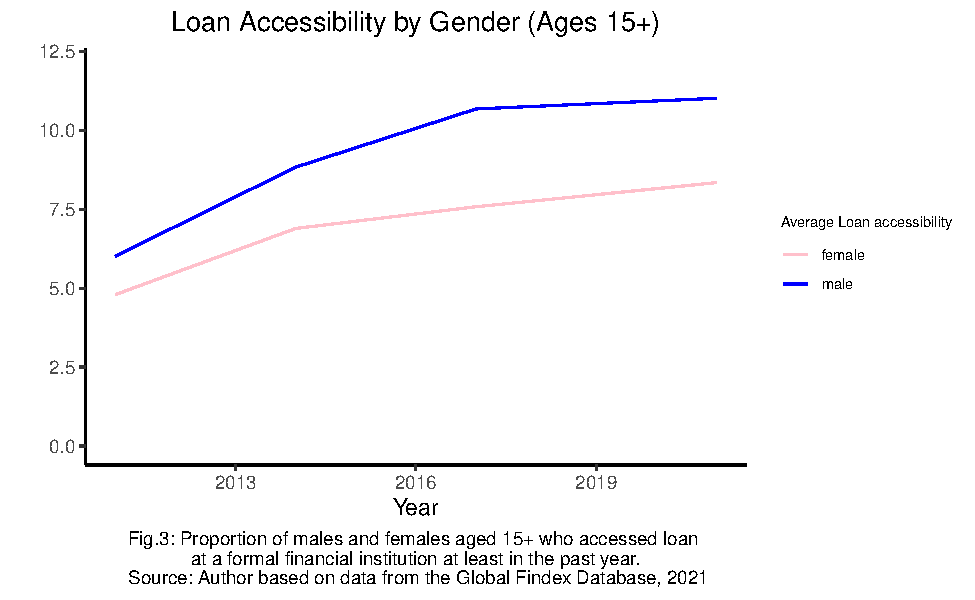
\includegraphics{504.Project1_files/figure-latex/unnamed-chunk-3-3.pdf}
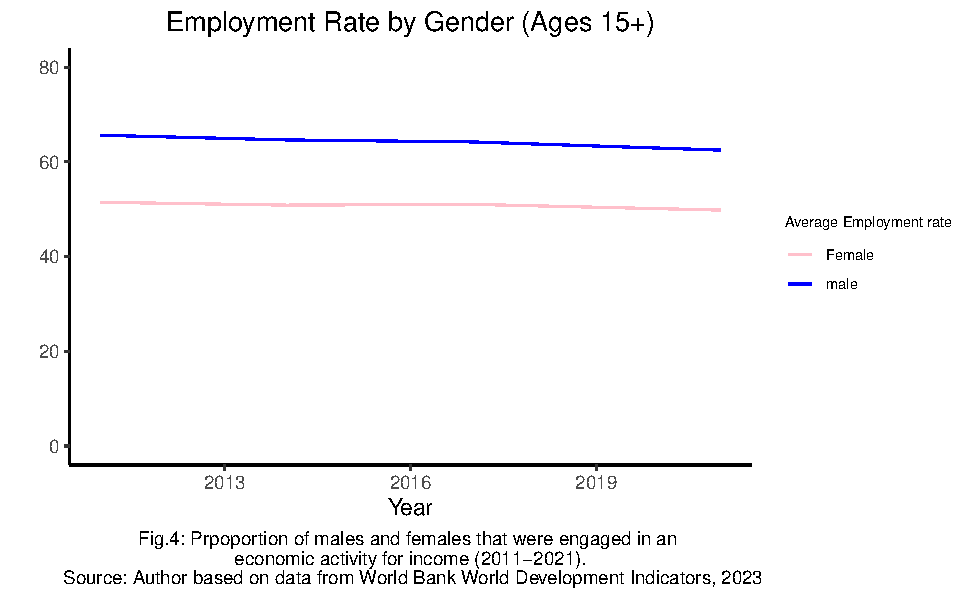
\includegraphics{504.Project1_files/figure-latex/unnamed-chunk-3-4.pdf}
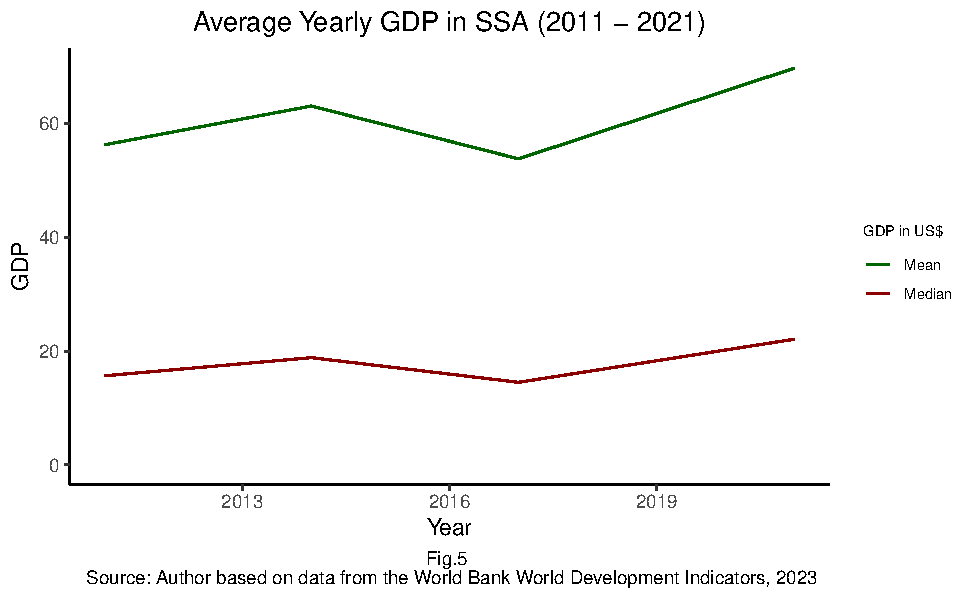
\includegraphics{504.Project1_files/figure-latex/unnamed-chunk-3-5.pdf}

\hypertarget{financial-inclusion-gender-gap-per-country}{%
\subsection{Financial Inclusion Gender Gap per
Country}\label{financial-inclusion-gender-gap-per-country}}

The financial inclusion gender gap was further examined in each of the
26 countries used in the study. The chloropleths below show that on
average, gender disparity is almost the same for most of the countries
with few countries showing significantly high and low values. For gender
gap in relation to account ownership shown in Fig6, majority of the SSA
countries have a gap above 10\% with only 7 (Ghana, Kenya, Zambia,
Namibia, Lesotho, Mauritius, and South Africa) recording gaps less than
10\%. South Africa most notably has a negative gap with the proportion
females about 0.4\% higher than males. Two countries however, Cote
d'Ivoire and Sudan have the highest account ownership gender gap (above
30\%), thus the proportion of males with formal financial institution
accounts is over 30\% higher than that of females. In relation to gender
gap in savings which is dsiplayed in fig7, the study found that the
majority of the countries (21 out of 26) have an average gender gap
above 10\% and only 6 (Namibia, Zambia, South Africa, Lesotho,
Madagascar, and Mauritius) recorded an average gap below 10\% with
Madagascar recording th lowest of 0.8\%. Sudan, Madagascar, and
Mozambique averagely recorded a gap greater than 30\%. This indicates
that on average the proportion of males who save some money in a year
are more than 10\% or more more than females in the SSA area. Examining
the gender gap associated with loan accessibility displayed in Fig8, it
was observed that just like the two gender gaps, most of the SSA
countries have similar gaps. Eight of the countries recorded a single
digit gap on average and the remaining 18 countries recorded average
loan gap greater than 10\%. Cote d'Ivoire, Gabon, and Mauritius on
average recorded more than 30\% average loan gender gap with Cote
d'Ivoire recording the highest of 43\%. Sierra Leone and Malawi recorded
gender gaps less than 0 which shows that in this countries more females
access loans than males. Thus, considering all the gender gaps together,
visuals show that in most of the countries in the Sub-Saharan Africa
region the proportion of males that have access to financial services is
on average over 10\% more than that of females.

\bigskip

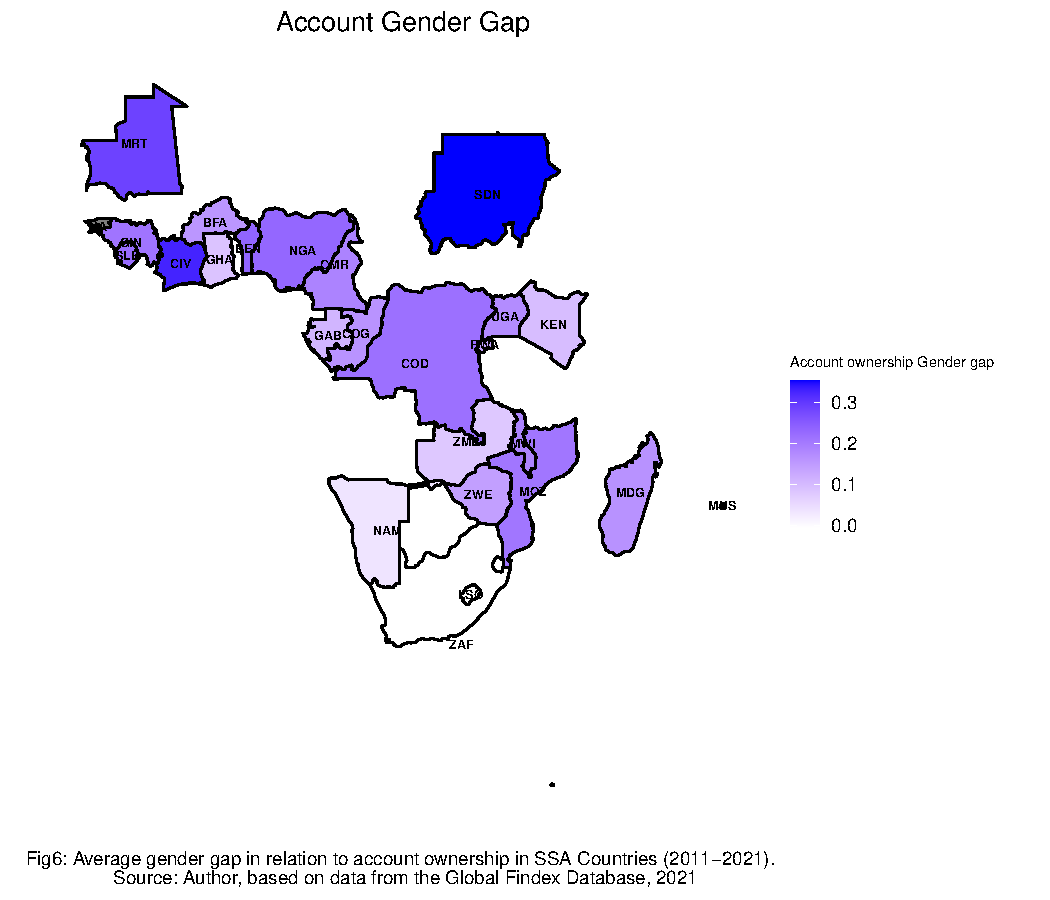
\includegraphics{504.Project1_files/figure-latex/unnamed-chunk-4-1.pdf}
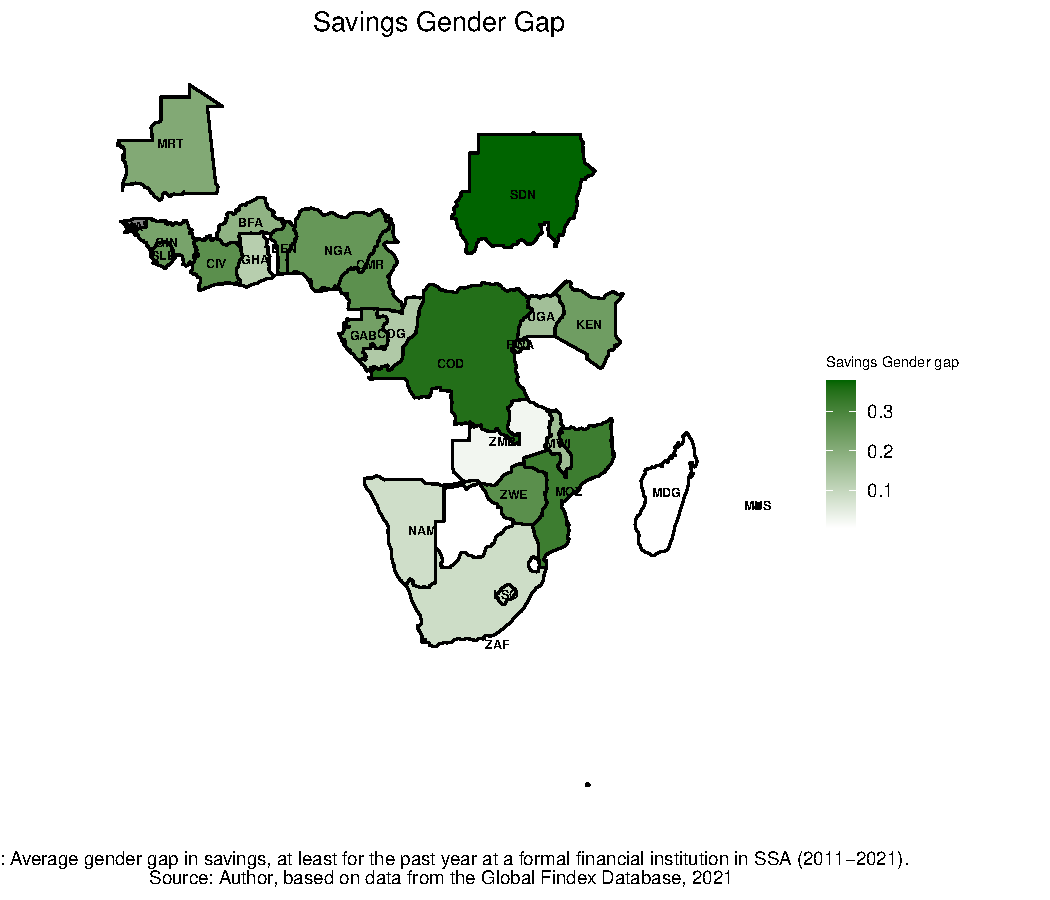
\includegraphics{504.Project1_files/figure-latex/unnamed-chunk-4-2.pdf}
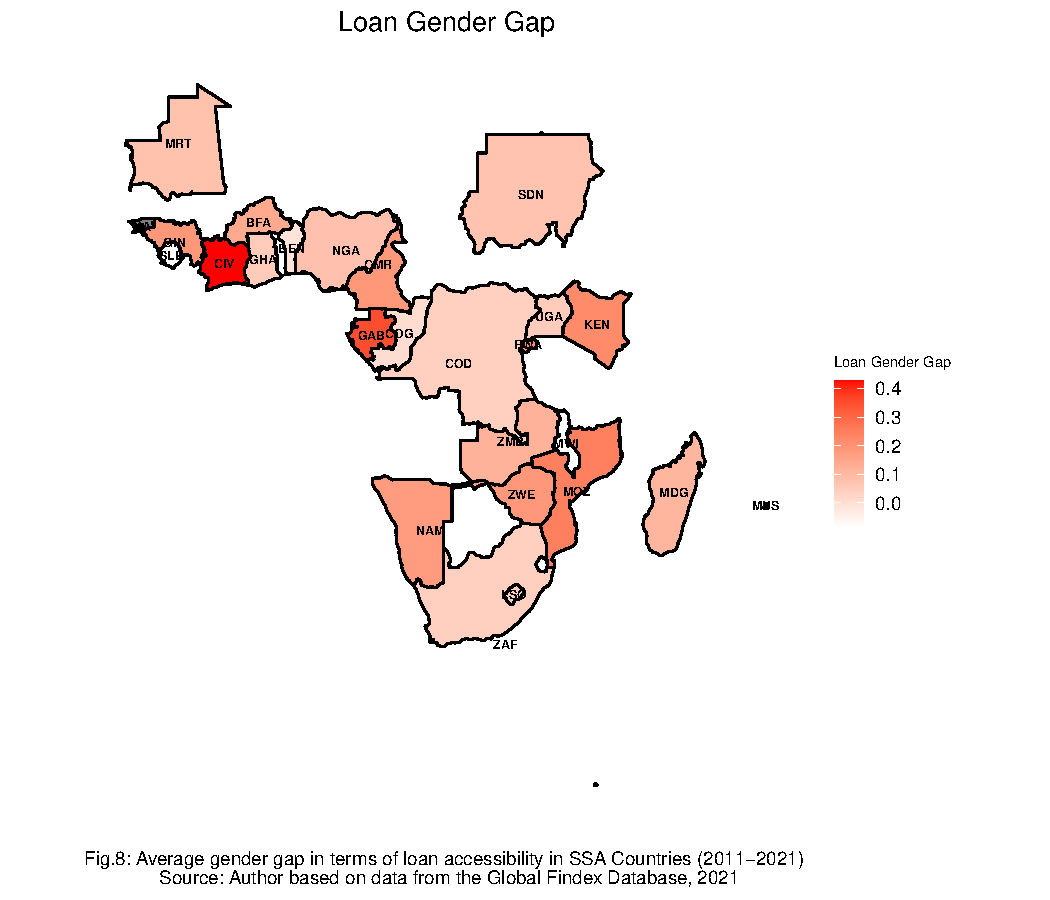
\includegraphics{504.Project1_files/figure-latex/unnamed-chunk-4-3.pdf}

\hypertarget{employment-gender-gap-per-country}{%
\subsection{Employment Gender Gap per
Country}\label{employment-gender-gap-per-country}}

Employment in the SSA region has been an issue for discussion over the
years as this tends to be one of the areas where gender disparity
appears to be significant. The study examined the gender disparity in
the 26 countries studied in this paper. It was found that 6 of the 26
countries have an average gender gap less than 10\%, most of the
countries have a gender gap between 10\% and 30\%, and 4 of the
countries have average gender gap greater than 50\%. The study found an
average gender gap of over 100 \% in Sudan and nearly 80\% in
Mauritania. This is shown in Fig9 below. This employment gender gap
tends to agree with the gender gap in financial inclusion shown above.

\bigskip

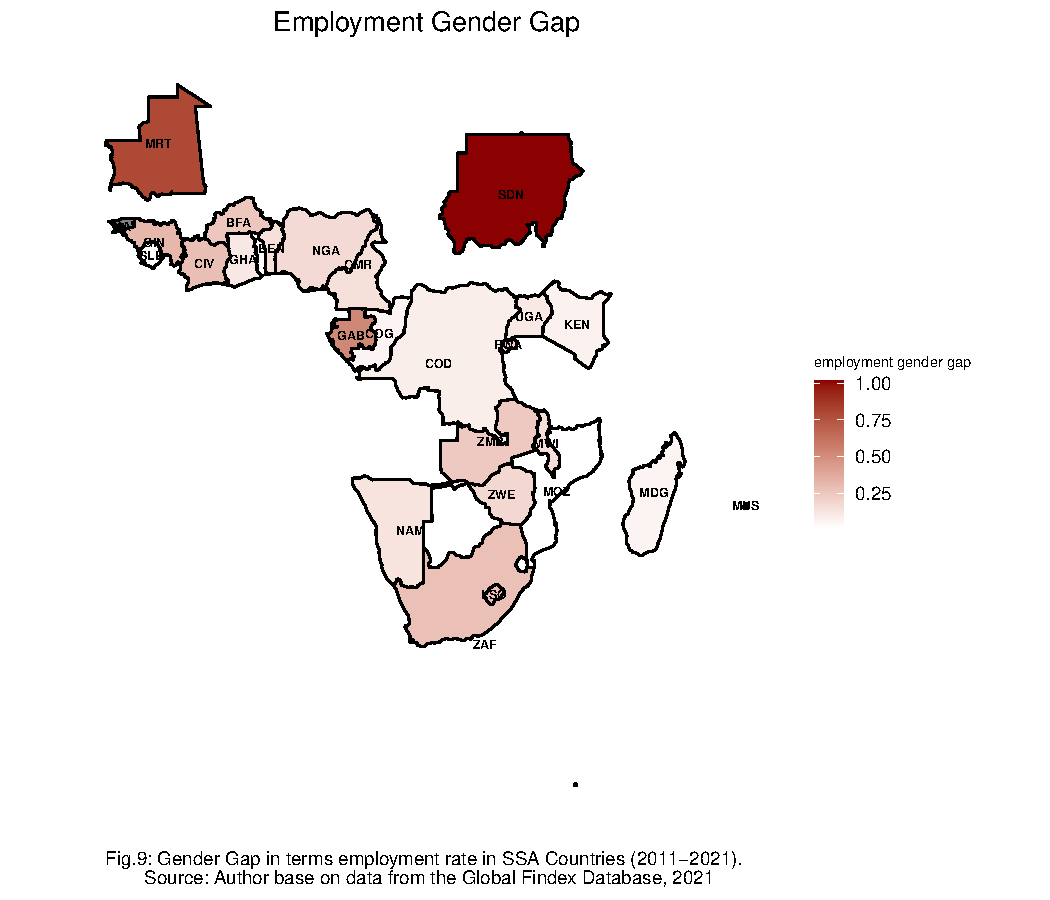
\includegraphics{504.Project1_files/figure-latex/unnamed-chunk-5-1.pdf}

\hypertarget{assessing-individual-fintech-variables}{%
\subsection{Assessing Individual Fintech
Variables}\label{assessing-individual-fintech-variables}}

The study further investigated the individual Fintech variables to
obtain better understanding of the Fintech ecosystem in the SSA region.
Fig10, Fig11, and Fig12 display bar plots that show the development of
access to internet, access to electricity and mobile subscriptions in
the region from 2011 to 2021 respectively. From the plots, it is
observed that internet access was less than 20\% for majority of the
countries in 2011. This progressed steadily over the years, however, as
at 2021, only 7 of the 26 countries have 50\% or more of their
population having access to internet. Similarly, in 2011, only 7 out of
the 26 countries had more than 50\% of its population having access to
electricity with Mauritius being the only country with nearly 100\%
electricity access. Apart from Mauritius which had nearly 100\% since
2011, access to electricity in the remaining countries developed
progressively, however, only 4 other countries had had at least 75\%
electricity access with Ghana, Gabon, and South Africa being well over
80\%. Mobile telephony subscription is the Fintech variable that is very
high in the region. As at 2014, only 3 of the 26 countries (Malawi,
Mozambique, and Madagascar) had mobile telephony subscription of less
than 50\% of its population. However, at the end of 2021, 14 of the 26
countries had over 100\% mobile telephony with only Mozambique and
Malawi recording lower than 50\% subscriptions. This indicates that the
use of mobile phone is very high in the SSA region despite the low
inyternet access and access to electricity. This suggests that on
average, the low access to internet and electricity is quite worrisome
for development of Fintech as Fintech development is impossible without
the availability of internet and electricity.

\bigskip

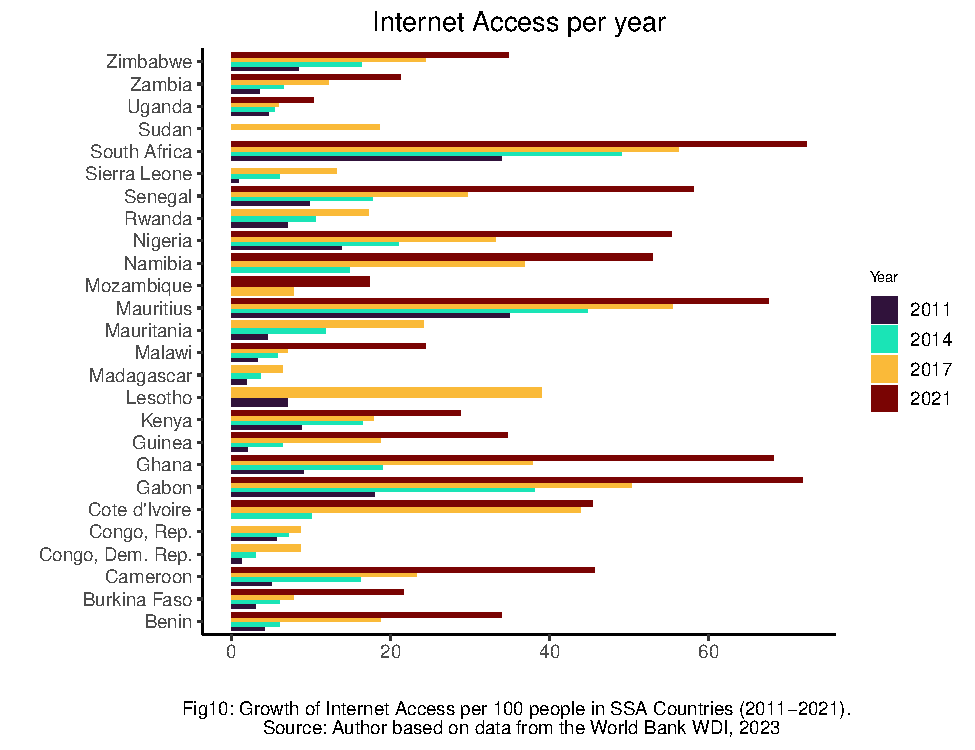
\includegraphics{504.Project1_files/figure-latex/unnamed-chunk-6-1.pdf}
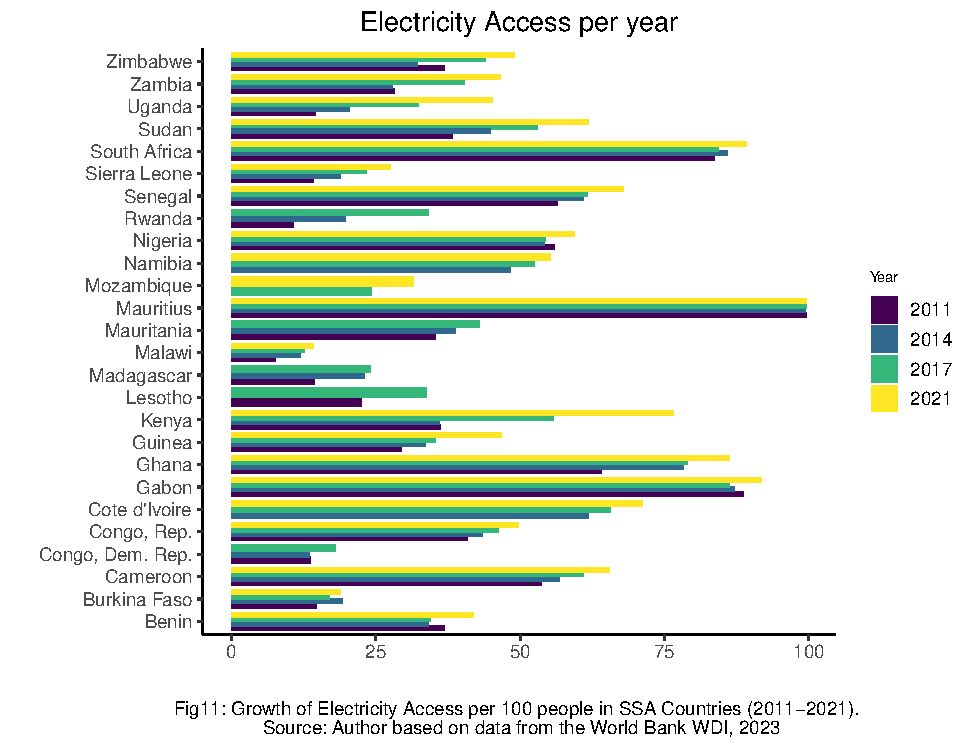
\includegraphics{504.Project1_files/figure-latex/unnamed-chunk-6-2.pdf}
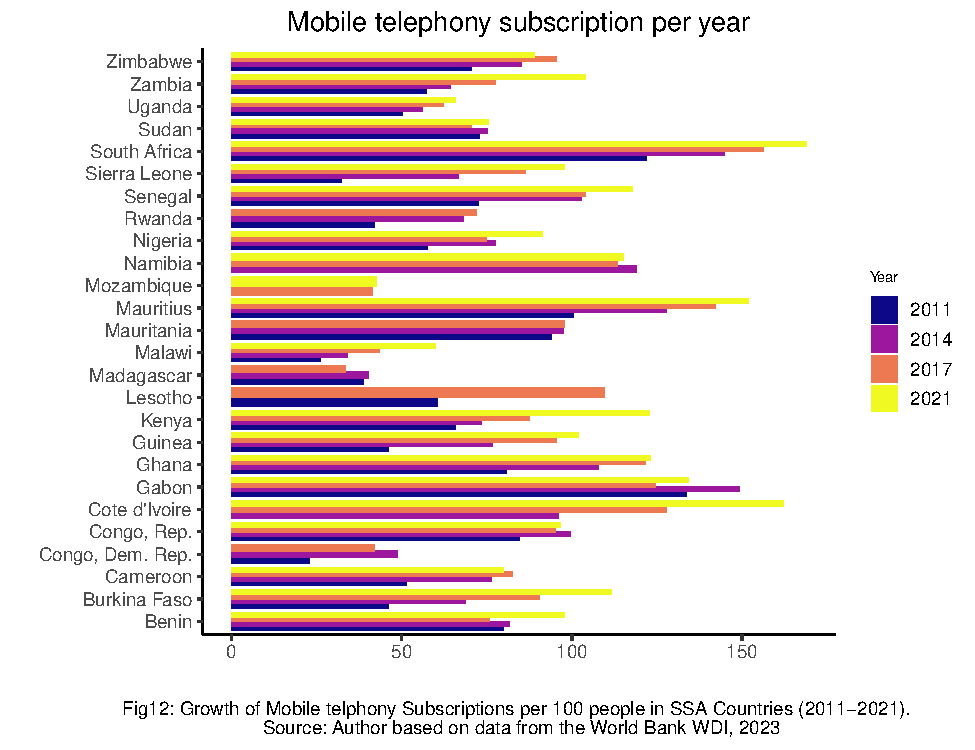
\includegraphics{504.Project1_files/figure-latex/unnamed-chunk-6-3.pdf}

\hypertarget{overall-fintech-development-in-ssa}{%
\subsection{Overall Fintech Development in
SSA}\label{overall-fintech-development-in-ssa}}

Fintech development in the 26 SSA countries studied was found to be low
on average with only 6 of the countries recording Fintech development of
over 50\%, the rest have an average value lower than 50\% according to
Fig13 below. The fact that 20 of the 26 SSA countries have comparatively
low average Fintech development highlights how young the Fintech sector
is in the area. Fintech's influence and development in Sub-Saharan
Africa are still developing, despite its increasing recognition on a
worldwide scale as a catalyst for innovation and financial inclusion.
Furthermore, the observation that Fintech development exceeded 50\% in
only six of the twenty-six SSA countries analysed demonstrates the
moderate variation in the adoption and progression of Fintech solutions
throughout the region. This indicates that factors including
technological readiness, regulatory environment, infrastructure, and
economic stability may make certain countries more favourable to Fintech
innovation. The prevalence of countries with less than 50\% Fintech
development suggests that numerous SSA countries face obstacles and
challenges that impede the expansion of the Fintech industry. Potential
obstacles may comprise regulatory limitations, restricted investment and
capital accessibility, insufficient digital infrastructure, and a dearth
of proficient personnel.

\bigskip

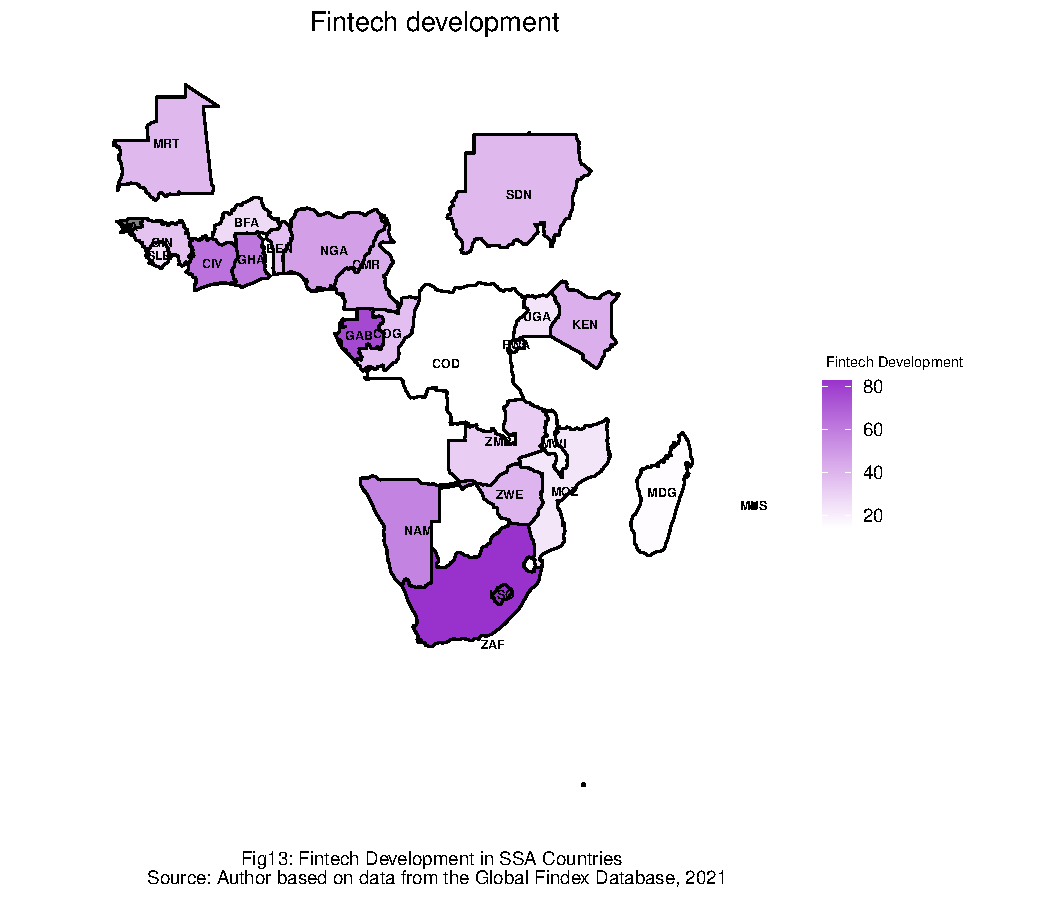
\includegraphics{504.Project1_files/figure-latex/unnamed-chunk-7-1.pdf}

\hypertarget{relationship-between-fintech-and-figg}{%
\subsection{Relationship between Fintech and
FIGG}\label{relationship-between-fintech-and-figg}}

In SSA, the study identifies from Fig14 a linear relationship between
FIGG variables and Fintech development. Fintech development in the
region has a negative linear relationship with the gender gap in account
ownership. This shows that when Fintech dvelopment increase in the area,
the gender gap in account ownership will decrease.This negative
relationship suggests that advancements in Fintech can contribute
positively to financial inclusion efforts, particularly in addressing
gender disparities in accessing financial services. It was further found
that the relationship is linear and positive between Fintech and the
gender gap in Loan accessibility as shown in Fig15. This positive
relationship between Fintech development and the gender gap in loan
accessibility indicates a concerning trend where increased Fintech
development is associated with a widening gap between males and females
in accessing formal financial institutions for loans. This could be as a
result of gender biases that may be embedded within the design and
implementation of Fintech products and services, leading to unequal
access to credit for women. Additionally, socio-economic factors such as
disparities in digital literacy, ownership of mobile phones or internet
access, and cultural norms that may disproportionately affect women's
ability to utilize Fintech solutions for accessing credit. Inadequate
access to credit can hinder women's ability to invest in education,
entrepreneurship, and productive assets, thereby perpetuating cycles of
poverty and inequality since most families are being managed by women
and most women are also single parents in the region.

In addition,there is nearly neutral relationship between Fintech and the
gender gap in Savings as seen in Fig16. wThis indicates that, while
there might be some relationship between Fintech development and the
gender gap in savings, it is not significant or substantial. In other
words, the impact of Fintech on the gender gap in savings is minimal or
negligible. This could mean that Fintech developments do not
specifically target or disproportionately affect savings behaviors or
access for either gender, or that other factors outweigh the influence
of Fintech in this regard.

\bigskip

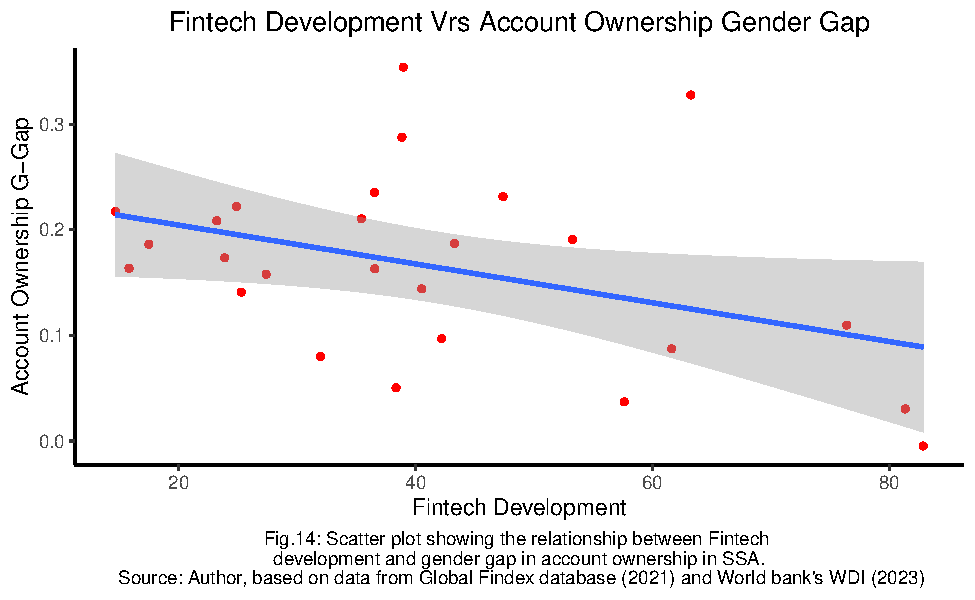
\includegraphics{504.Project1_files/figure-latex/unnamed-chunk-8-1.pdf}
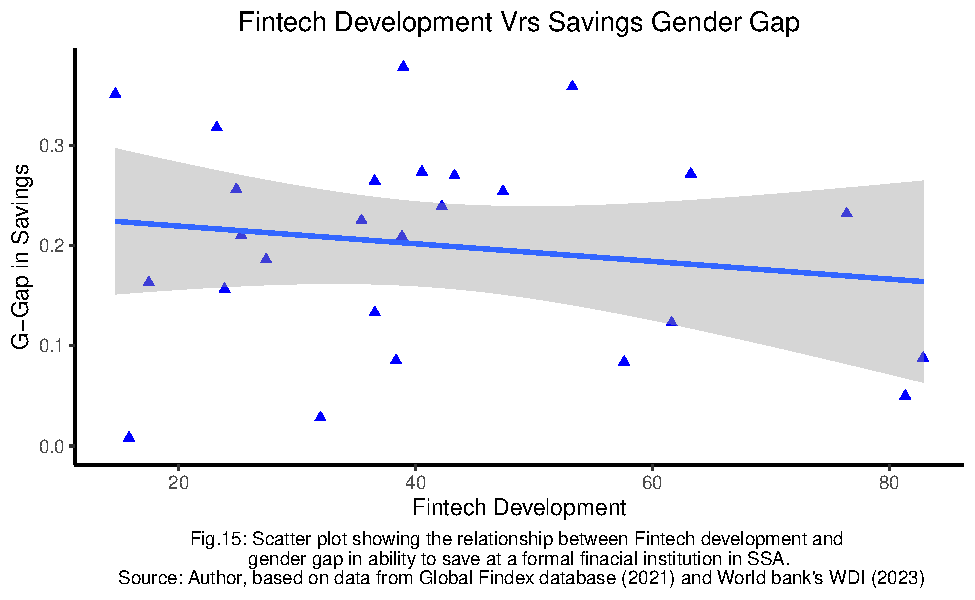
\includegraphics{504.Project1_files/figure-latex/unnamed-chunk-8-2.pdf}
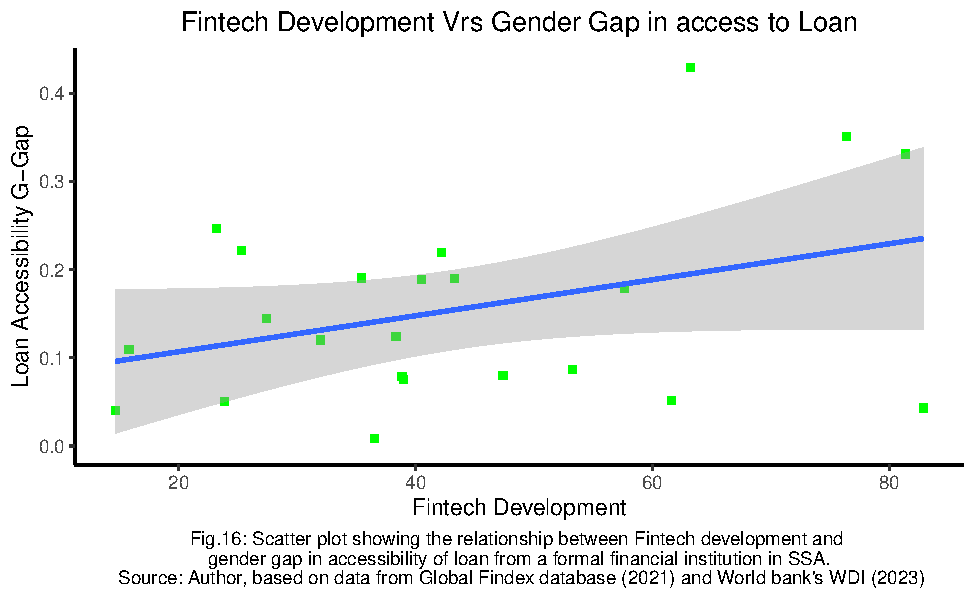
\includegraphics{504.Project1_files/figure-latex/unnamed-chunk-8-3.pdf}

\hypertarget{population-growth-by-gender}{%
\subsection{Population growth by
Gender}\label{population-growth-by-gender}}

Since the denominator for the proportion of both males and females with
access to financial services is the number of males and females aged 15+
respectively, the study investigated the magnitude of the difference in
the growth of the population for both groups. This was done to better
understand if the difference in proportions could also be explained by
the difference in population in both groups. Upon investigating this, it
is shown in Fig17 and Fig18 that the proportion of males and females
aged 15 and above have had almost similar growth rates over the periods
of study. In Fig19, the male proportion and female proportion for each
country in the year 2021 was displayed together to observe the magnitude
of the difference between the groups. The plot showed that although all
the countries had more females than males, the difference between the
proportions is fairly below 5\% for all the countries with Zimbabwe
recording the highest of about 4\%. This suggests that population
difference could not neccessarily be the reason for the gender disparity
in terms of access to financial services, which is referred to as
financial inclusion gender gap.

\bigskip

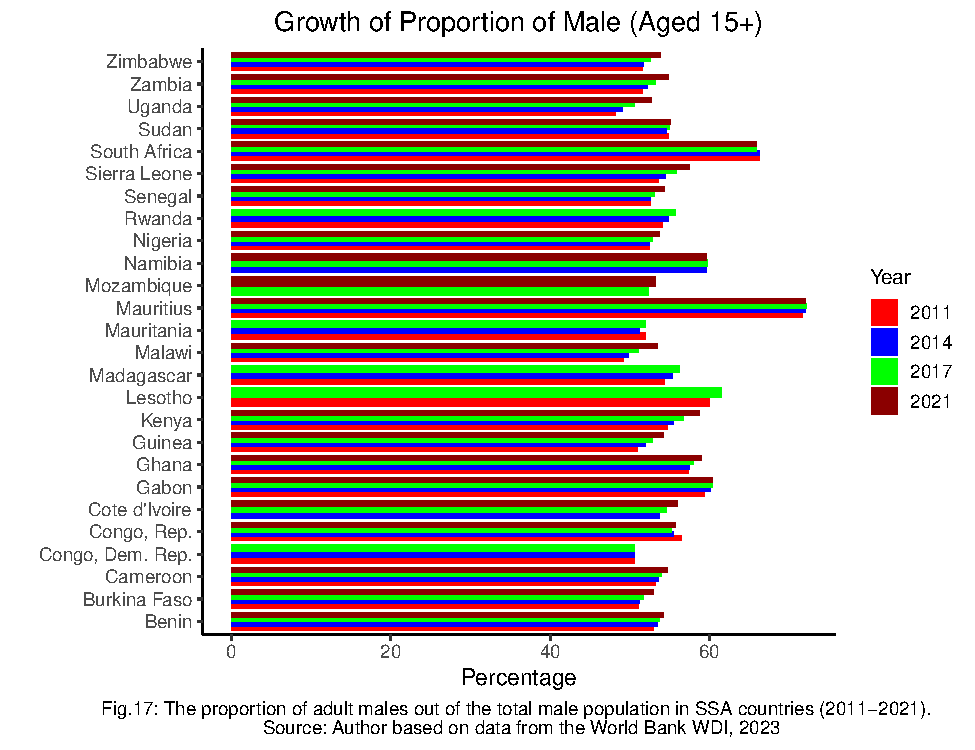
\includegraphics{504.Project1_files/figure-latex/unnamed-chunk-9-1.pdf}
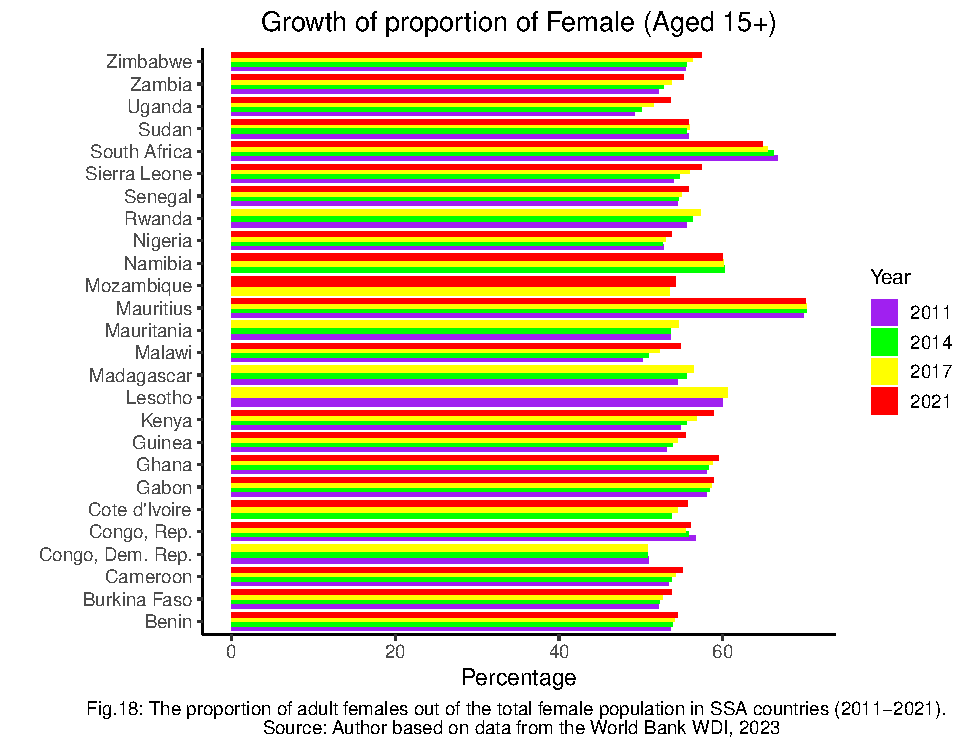
\includegraphics{504.Project1_files/figure-latex/unnamed-chunk-9-2.pdf}
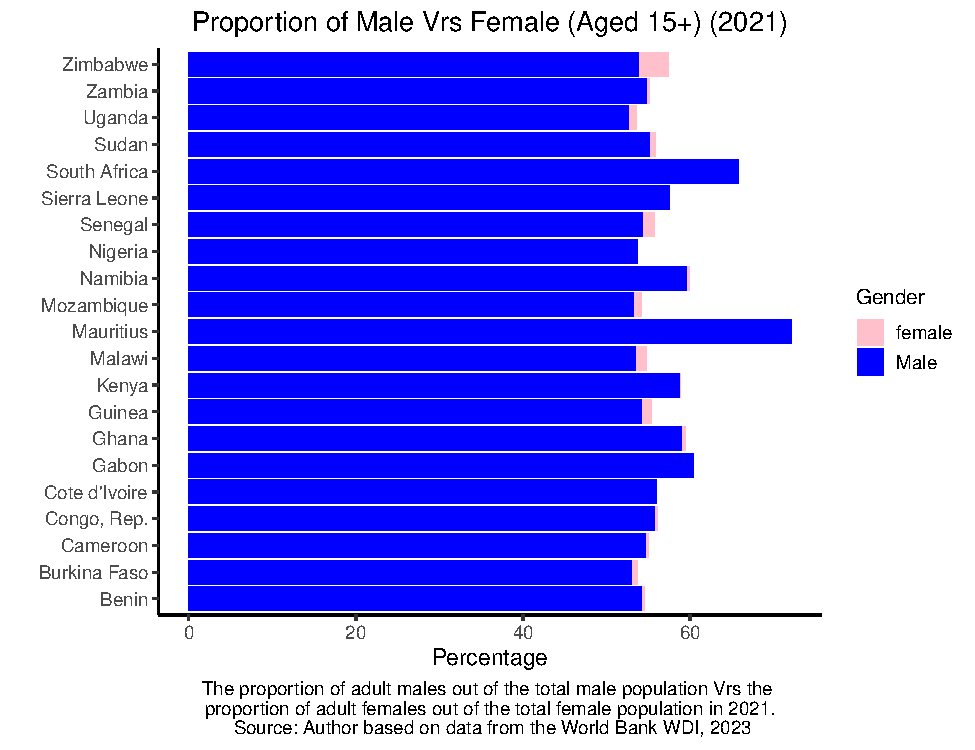
\includegraphics{504.Project1_files/figure-latex/unnamed-chunk-9-3.pdf}

\hypertarget{conclusion}{%
\section{CONCLUSION}\label{conclusion}}

Notwithstanding the present limited developments in Fintech, there is
cause for optimism regarding the potential for future expansion and
influence. With the growing recognition and interest in digital
financial services, coupled with technological advancements and
increased investment in this domain, Sub-Saharan African countries (SSA)
possess the capacity to surpass conventional banking models by adopting
inventive Fintech solutions that address the distinct requirements and
inclinations of their populace.

In light of the pivotal significance that Fintech possesses in fostering
economic expansion, financial inclusion, and digital revolution, it is
imperative to accord top priority to the establishment of resilient
Fintech ecosystems in Sub-Saharan African nations. This entails
addressing broader ecosystem enablers, including but not limited to
supportive regulatory frameworks, access to funding and venture capital,
digital literacy and skills development, and partnerships among
governments, financial institutions, technology firms, and other
stakeholders, in addition to fostering technological innovation. In
brief, although the results indicate that Fintech progress in
Sub-Saharan African nations is presently limited, they also emphasize
the tremendous potential that Fintech has to facilitate inclusive
economic expansion, enhance financial accessibility, and enable both
individuals and enterprises throughout the area---given that the
requisite conditions and support systems are established. Emphasizing
the importance of fostering an environment conducive to Fintech
development to reduce gender inequalities in financial access. This may
involve supporting regulatory frameworks that promote innovation and
ensuring that Fintech solutions are accessible and tailored to the needs
of marginalised populations, including women.

It must be noted that this analysis is made solely based on data from
the 26 Sub-Saharan African countries and the visualizations produced in
the study, thus, generalization of findings must be done with caution.
Further empirical analysis would b required to provide sufficient
evidence and explanation to the study concept.

\bibliography{mybibfile.bib}


\end{document}
